\documentclass{beamer}
\usetheme{Warsaw}

\usepackage[utf8]{inputenc}
\usepackage[T1]{fontenc}
\usepackage{fancybox}
\usepackage{multimedia} 
\usepackage{subfig}
\usepackage{amsmath}
\usepackage{amssymb}
\usepackage{hyperref}
\hypersetup{
    colorlinks=true,     
    urlcolor=blue
}
\usepackage[all]{xy}
\usepackage{tikz}
\usetikzlibrary{automata, positioning, arrows}
\setbeamertemplate{footline}[frame number]

\newcommand{\R}{\mathbb{R}}
\newcommand{\N}{\mathbb{N}}
\newcommand{\E}{\mathbb{E}}
\newcommand{\PP}{\mathbb{P}}

\begin{document}


\title[Stochastik] % (optional, only for long titles)
{Wahrscheinlichkeitstheorie und Statistik (Stochastik)
\\
Markov-Ketten
}
\subtitle{}
\author[Dr. Johannes Riesterer] % (optional, for multiple authors)
{Dr.  rer. nat. Johannes Riesterer}

\date[KPT 2004] % (optional)
{}

\subject{Stochastik}

\frame{\titlepage}


%% =============================================
%% MOTIVATION
%% =============================================

\begin{frame}
    \frametitle{Markov-Ketten}
\framesubtitle{Motivation}
    \begin{block}{Idee}
Viele Prozesse in der Informatik und im Alltag können als Folge von Zuständen modelliert werden, bei denen der nächste Zustand nur vom aktuellen Zustand abhängt -- nicht von der gesamten Vergangenheit.
\end{block}
\pause
\begin{block}{Beispiele}
\begin{itemize}
\item Websurfen: Die nächste Seite hängt nur von der aktuellen Seite ab (PageRank).
\item Wetter: Morgen Regen/Sonne hängt (vereinfacht) nur vom heutigen Wetter ab.
\item Warteschlangen: Anzahl der Kunden hängt nur vom aktuellen Zustand ab.
\end{itemize}
\end{block}
 \end{frame}


%% =============================================
%% DEFINITION STOCHASTISCHE MATRIX
%% =============================================

\begin{frame}
    \frametitle{Markov-Ketten}
\framesubtitle{Stochastische Matrix}
    \begin{block}{Definition (Stochastische Matrix)}
Eine Matrix $P = (p_{ij})_{i,j \in S}$ mit Zustandsraum $S$ heißt \textbf{stochastische Matrix}, falls:
\begin{enumerate}
\item $p_{ij} \geq 0$ für alle $i, j \in S$
\item $\sum_{j \in S} p_{ij} = 1$ für alle $i \in S$ \quad (Zeilensumme = 1)
\end{enumerate}
\end{block}
\pause
\begin{block}{Interpretation}
$p_{ij}$ ist die Wahrscheinlichkeit, vom Zustand $i$ in den Zustand $j$ zu wechseln.
\end{block}
 \end{frame}


%% =============================================
%% LEAN: STOCHASTISCHE MATRIX
%% =============================================

\begin{frame}[fragile]
    \frametitle{Markov-Ketten}
\framesubtitle{Lean -- Stochastische Matrix}
    \begin{block}{Formalisierung in Lean 4 / Mathlib}
\begin{verbatim}
abbrev S (N : Nat) := Fin N

def IsTransitionMatrix (P : S N -> S N -> Real) : Prop :=
  (forall x y, 0 <= P x y) /\
  (forall x, (Sum y, P x y) = 1)
\end{verbatim}
\end{block}
\pause
\begin{block}{Korrespondenz}
\begin{tabular}{lcl}
$S = \{1, \ldots, N\}$ & $\longleftrightarrow$ & \texttt{Fin N} \\
$p_{ij} \geq 0$ & $\longleftrightarrow$ & \texttt{$\forall$ x y, 0 $\leq$ P x y} \\
$\sum_j p_{ij} = 1$ & $\longleftrightarrow$ & \texttt{$\forall$ x, ($\sum$ y, P x y) = 1}
\end{tabular}
\end{block}
 \end{frame}


%% =============================================
%% BEISPIEL: 2 ZUSTÄNDE (WETTER)
%% =============================================

\begin{frame}
    \frametitle{Markov-Ketten}
\framesubtitle{Beispiel: Wetter mit 2 Zuständen}
    \begin{block}{Zustandsraum}
$S = \{S(\text{onne}), R(\text{egen})\}$
\end{block}

\begin{center}
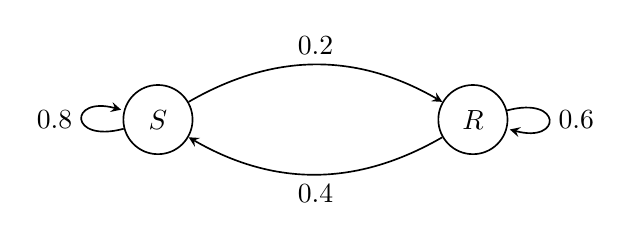
\begin{tikzpicture}[->, >=stealth, auto, semithick, node distance=4cm]
    \node[state] (S) {$S$};
    \node[state] (R) [right of=S] {$R$};
    \path (S) edge[loop left] node{$0.8$} (S)
              edge[bend left] node{$0.2$} (R)
          (R) edge[bend left] node{$0.4$} (S)
              edge[loop right] node{$0.6$} (R);
\end{tikzpicture}
\end{center}

\begin{block}{Übergangsmatrix}
\[
P = \begin{pmatrix} 0.8 & 0.2 \\ 0.4 & 0.6 \end{pmatrix}
\]
Zeile 1: Wenn heute Sonne, dann morgen Sonne mit $0.8$, Regen mit $0.2$.
\end{block}
 \end{frame}


%% =============================================
%% LEAN: WETTER-BEISPIEL
%% =============================================

\begin{frame}[fragile]
    \frametitle{Markov-Ketten}
\framesubtitle{Lean -- Wetter-Beispiel}
    \begin{block}{Konkrete Definition in Lean}
\begin{verbatim}
def weatherP : S 2 -> S 2 -> Real
  | <0, _>, <0, _> => 0.8
  | <0, _>, <1, _> => 0.2
  | <1, _>, <0, _> => 0.4
  | <1, _>, <1, _> => 0.6
\end{verbatim}
\end{block}
\pause
\begin{block}{Beweis: weatherP ist stochastische Matrix}
\begin{verbatim}
lemma weatherP_isTransition :
    IsTransitionMatrix weatherP := by
  constructor
  . intro x y
    fin_cases x <;> fin_cases y <;>
      simp [weatherP] <;> norm_num
  . intro x
    fin_cases x <;> simp [weatherP] <;> norm_num
\end{verbatim}
\end{block}
 \end{frame}


%% =============================================
%% DEFINITION MARKOV-KETTE
%% =============================================

\begin{frame}
    \frametitle{Markov-Ketten}
\framesubtitle{Definition}
    \begin{block}{Definition (Markov-Kette)}
Eine Folge von Zufallsvariablen $(X_n)_{n \in \N_0}$ mit Werten in einem abzählbaren Zustandsraum $S$ heißt \textbf{Markov-Kette} mit Übergangsmatrix $P$, falls:
\[
\PP(X_{n+1} = j \mid X_n = i, X_{n-1} = i_{n-1}, \ldots, X_0 = i_0) = \PP(X_{n+1} = j \mid X_n = i) = p_{ij}
\]
für alle $n \in \N_0$ und alle $i, j, i_0, \ldots, i_{n-1} \in S$.
\end{block}
\pause
\begin{block}{Markov-Eigenschaft (Gedächtnislosigkeit)}
Die Zukunft hängt nur von der Gegenwart ab, nicht von der Vergangenheit!
\end{block}
 \end{frame}


%% =============================================
%% LEAN: MARKOV-EIGENSCHAFT
%% =============================================

\begin{frame}[fragile]
    \frametitle{Markov-Ketten}
\framesubtitle{Lean -- Markov-Eigenschaft}
    \begin{block}{Formalisierung über bedingte Erwartung}
\begin{verbatim}
noncomputable def stepOp (P : S N -> S N -> Real)
    (f : S N -> Real) : S N -> Real :=
  fun x => Sum y, P x y * f y

def IsHomogeneousMarkov (mu : Measure Omega)
    (F : Filtration Nat _) (X : Nat -> Omega -> S N)
    (P : S N -> S N -> Real) : Prop :=
  Adapted F X /\
  forall n (f : S N -> Real), Measurable f ->
    mu[fun w => f (X (n+1) w)|F n] =a.e.[mu]
      fun w => stepOp P f (X n w)
\end{verbatim}
\end{block}
\pause
\begin{block}{Bedeutung}
$\E[f(X_{n+1}) | \mathcal{F}_n] = (Pf)(X_n)$ \quad fast sicher.\\
Dies ist die maßtheoretische Version der Markov-Eigenschaft.
\end{block}
 \end{frame}


%% =============================================
%% BEISPIEL: 3 ZUSTÄNDE
%% =============================================

\begin{frame}
    \frametitle{Markov-Ketten}
\framesubtitle{Beispiel: 3 Zustände (Stimmung)}
    \begin{block}{Modell}
$S = \{G(\text{ut}), N(\text{eutral}), S(\text{chlecht})\}$
\end{block}

\begin{center}
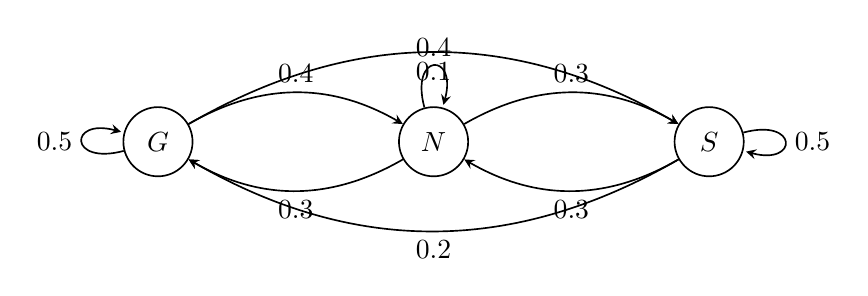
\begin{tikzpicture}[->, >=stealth, auto, semithick, node distance=3.5cm]
    \node[state] (G) {$G$};
    \node[state] (N) [right of=G] {$N$};
    \node[state] (S) [right of=N] {$S$};
    \path (G) edge[loop left] node{$0.5$} (G)
              edge[bend left] node{$0.4$} (N)
              edge[bend left] node[below]{$0.1$} (S)
          (N) edge[bend left] node{$0.3$} (G)
              edge[loop above] node{$0.4$} (N)
              edge[bend left] node{$0.3$} (S)
          (S) edge[bend left] node[below]{$0.2$} (G)
              edge[bend left] node{$0.3$} (N)
              edge[loop right] node{$0.5$} (S);
\end{tikzpicture}
\end{center}

\[
P = \begin{pmatrix} 0.5 & 0.4 & 0.1 \\ 0.3 & 0.4 & 0.3 \\ 0.2 & 0.3 & 0.5 \end{pmatrix}
\]
 \end{frame}


%% =============================================
%% n-SCHRITT ÜBERGANGSWAHRSCHEINLICHKEITEN
%% =============================================

\begin{frame}
    \frametitle{Markov-Ketten}
\framesubtitle{$n$-Schritt Übergangswahrscheinlichkeiten}
    \begin{block}{Satz (Chapman-Kolmogorov)}
Die Wahrscheinlichkeit, in $n$ Schritten von $i$ nach $j$ zu gelangen, ist:
\[
p_{ij}^{(n)} = \PP(X_n = j \mid X_0 = i) = (P^n)_{ij}
\]
Also: Einfach die Matrix $n$-mal mit sich selbst multiplizieren!
\end{block}
\pause
\begin{block}{Beispiel (Wetter)}
Wie ist das Wetter übermorgen, wenn heute Sonne?
\[
P^2 = \begin{pmatrix} 0.8 & 0.2 \\ 0.4 & 0.6 \end{pmatrix}^2 = \begin{pmatrix} 0.72 & 0.28 \\ 0.56 & 0.44 \end{pmatrix}
\]
$\Rightarrow$ Wahrscheinlichkeit für Sonne übermorgen: $0.72$.
\end{block}
 \end{frame}


%% =============================================
%% LEAN: MATRIXPOTENZ
%% =============================================

\begin{frame}[fragile]
    \frametitle{Markov-Ketten}
\framesubtitle{Lean -- Matrixpotenz}
    \begin{block}{Rekursive Definition}
\begin{verbatim}
noncomputable def matMul (P Q : S N -> S N -> Real) :=
  fun x z => Sum y, P x y * Q y z

noncomputable def matPow (P : S N -> S N -> Real) :
    Nat -> S N -> S N -> Real
  | 0     => fun x z => if x = z then 1 else 0
  | n + 1 => matMul (matPow P n) P
\end{verbatim}
\end{block}
\pause
\begin{block}{Korrespondenz}
\begin{tabular}{lcl}
$P^0 = I$ (Einheitsmatrix) & $\longleftrightarrow$ & \texttt{if x = z then 1 else 0} \\
$P^{n+1} = P^n \cdot P$ & $\longleftrightarrow$ & \texttt{matMul (matPow P n) P} \\
$(P^n)_{xz} = \sum_y P^n_{xy} P_{yz}$ & $\longleftrightarrow$ & \texttt{$\sum$ y, P x y * Q y z}
\end{tabular}
\end{block}
 \end{frame}


%% =============================================
%% VERTEILUNG ZUM ZEITPUNKT n
%% =============================================

\begin{frame}
    \frametitle{Markov-Ketten}
\framesubtitle{Verteilung zum Zeitpunkt $n$}
    \begin{block}{Anfangsverteilung}
Die Verteilung von $X_0$ wird als \textbf{Anfangsverteilung} $\mu_0$ bezeichnet:
\[
\mu_0(i) = \PP(X_0 = i), \quad i \in S
\]
Als Zeilenvektor: $\mu_0 = (\mu_0(1), \mu_0(2), \ldots)$
\end{block}
\pause
\begin{block}{Verteilung nach $n$ Schritten}
\[
\mu_n = \mu_0 \cdot P^n
\]
\end{block}
\pause
\begin{block}{Beispiel (Wetter)}
Start: $\mu_0 = (1, 0)$ (heute sicher Sonne). Nach 2 Tagen:
\[
\mu_2 = (1, 0) \cdot P^2 = (0.72, \; 0.28)
\]
\end{block}
 \end{frame}


%% =============================================
%% INVARIANTE VERTEILUNG - DEFINITION
%% =============================================

\begin{frame}
    \frametitle{Markov-Ketten}
\framesubtitle{Invariante (stationäre) Verteilung -- Definition}
    \begin{block}{Definition (Invariante Verteilung)}
Ein Wahrscheinlichkeitsvektor $\pi = (\pi_1, \pi_2, \ldots)$ heißt \textbf{invariante} (oder \textbf{stationäre}) \textbf{Verteilung} der Markov-Kette mit Übergangsmatrix $P$, falls:
\[
\pi \cdot P = \pi
\]
d.h. $\pi$ ist ein Linkseigenvektor von $P$ zum Eigenwert $1$.
\end{block}
\pause
\begin{block}{Interpretation}
Startet die Kette mit Verteilung $\pi$, so bleibt die Verteilung für alle Zeiten $\pi$:
\[
\mu_0 = \pi \;\Rightarrow\; \mu_n = \pi \cdot P^n = \pi \quad \text{für alle } n.
\]
Das System befindet sich im ``Gleichgewicht''.
\end{block}
 \end{frame}


%% =============================================
%% LEAN: INVARIANTE VERTEILUNG
%% =============================================

\begin{frame}[fragile]
    \frametitle{Markov-Ketten}
\framesubtitle{Lean -- Invariante Verteilung}
    \begin{block}{Definitionen in Lean}
\begin{verbatim}
def IsDistribution (pi : S N -> Real) : Prop :=
  (forall i, 0 <= pi i) /\ (Sum i, pi i) = 1

def IsInvariant (P : S N -> S N -> Real)
    (pi : S N -> Real) : Prop :=
  forall j, (Sum i, pi i * P i j) = pi j
\end{verbatim}
\end{block}
\pause
\begin{block}{Korrespondenz}
\[
(\pi P)_j = \sum_i \pi_i \cdot P_{ij} = \pi_j \quad \longleftrightarrow \quad \texttt{$\forall$ j, ($\sum$ i, $\pi$ i * P i j) = $\pi$ j}
\]
Man beachte: Die Summe $\sum_i \pi_i P_{ij}$ über die Spalte $j$ entspricht der Linksmultiplikation $\pi P$.
\end{block}
 \end{frame}


%% =============================================
%% BEISPIEL: INVARIANTE VERTEILUNG BERECHNEN
%% =============================================

\begin{frame}
    \frametitle{Markov-Ketten}
\framesubtitle{Beispiel: Invariante Verteilung berechnen}
    \begin{block}{Wetter-Beispiel}
Gesucht: $\pi = (\pi_S, \pi_R)$ mit $\pi P = \pi$ und $\pi_S + \pi_R = 1$.
\end{block}
\pause
\begin{align*}
\pi P = \pi &\Leftrightarrow \begin{cases} 0.8 \pi_S + 0.4 \pi_R = \pi_S \\ 0.2 \pi_S + 0.6 \pi_R = \pi_R \end{cases} \\
&\Leftrightarrow \begin{cases} -0.2 \pi_S + 0.4 \pi_R = 0 \\ 0.2 \pi_S - 0.4 \pi_R = 0 \end{cases} \\
&\Leftrightarrow \pi_S = 2 \pi_R
\end{align*}
\pause
Mit $\pi_S + \pi_R = 1$: \quad $2\pi_R + \pi_R = 1$ \quad $\Rightarrow$ \quad $\pi_R = \frac{1}{3}$, \quad $\pi_S = \frac{2}{3}$.

\[
\boxed{\pi = \left(\frac{2}{3}, \frac{1}{3}\right)}
\]

\textbf{Interpretation:} Langfristig ist es $2/3$ der Zeit sonnig und $1/3$ der Zeit regnerisch.
 \end{frame}


%% =============================================
%% LEAN: INVARIANZ VERIFIZIEREN
%% =============================================

\begin{frame}[fragile]
    \frametitle{Markov-Ketten}
\framesubtitle{Lean -- Invarianz verifizieren}
    \begin{block}{Definition und Beweis in Lean}
\begin{verbatim}
def weatherPi : S 2 -> Real
  | <0, _> => 2/3
  | <1, _> => 1/3

lemma weatherPi_isInvariant :
    IsInvariant weatherP weatherPi := by
  intro j
  fin_cases j <;>
    simp [weatherP, weatherPi, Fin.sum_univ_two]
    <;> ring
\end{verbatim}
\end{block}
\pause
\begin{block}{Was passiert hier?}
\begin{itemize}
\item \texttt{fin\_cases j}: Fallunterscheidung über $j \in \{0, 1\}$.
\item \texttt{simp}: Vereinfacht die Summe $\sum_{i} \pi_i P_{ij}$.
\item \texttt{ring}: Verifiziert die arithmetische Gleichung.
\end{itemize}
\end{block}
 \end{frame}


%% =============================================
%% IRREDUZIBILITÄT
%% =============================================

\begin{frame}
    \frametitle{Markov-Ketten}
\framesubtitle{Irreduzibilität}
    \begin{block}{Definition (Irreduzibel)}
Eine Markov-Kette heißt \textbf{irreduzibel}, falls man von jedem Zustand $i$ jeden anderen Zustand $j$ mit positiver Wahrscheinlichkeit in endlich vielen Schritten erreichen kann:
\[
\forall\, i,j \in S \;\exists\, n \geq 1: \quad p_{ij}^{(n)} > 0
\]
\end{block}
\pause
\begin{columns}
\begin{column}{0.5\textwidth}
\begin{center}
\textbf{Irreduzibel:}\\[0.3cm]
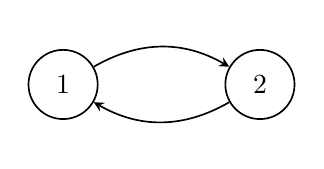
\begin{tikzpicture}[->, >=stealth, auto, semithick, node distance=2.5cm, scale=0.8]
    \node[state] (1) {$1$};
    \node[state] (2) [right of=1] {$2$};
    \path (1) edge[bend left] node{} (2)
          (2) edge[bend left] node{} (1);
\end{tikzpicture}
\end{center}
\end{column}
\begin{column}{0.5\textwidth}
\begin{center}
\textbf{Nicht irreduzibel:}\\[0.3cm]
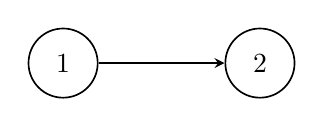
\begin{tikzpicture}[->, >=stealth, auto, semithick, node distance=2.5cm, scale=0.8]
    \node[state] (1) {$1$};
    \node[state] (2) [right of=1] {$2$};
    \path (1) edge node{} (2);
\end{tikzpicture}
\end{center}
\end{column}
\end{columns}
\vspace{0.3cm}
\textbf{Interpretation:} Alle Zustände ``kommunizieren'' miteinander.
 \end{frame}


%% =============================================
%% LEAN: IRREDUZIBILITÄT
%% =============================================

\begin{frame}[fragile]
    \frametitle{Markov-Ketten}
\framesubtitle{Lean -- Irreduzibilität}
    \begin{block}{Definition in Lean}
\begin{verbatim}
def IsIrreducible (P : S N -> S N -> Real) : Prop :=
  forall i j, exists n, 0 < n /\ 0 < matPow P n i j
\end{verbatim}
\end{block}
\pause
\begin{block}{Beweis: Wetter-Kette ist irreduzibel}
\begin{verbatim}
lemma weatherP_irreducible :
    IsIrreducible weatherP := by
  intro i j
  exact <1, Nat.one_pos, by
    fin_cases i <;> fin_cases j <;>
      simp [matPow, matMul, weatherP,
            Fin.sum_univ_two] <;> norm_num>
\end{verbatim}
\end{block}
Alle Einträge von $P^1$ sind positiv $\Rightarrow$ jeder Zustand ist in einem Schritt erreichbar.
 \end{frame}


%% =============================================
%% APERIODIZITÄT
%% =============================================

\begin{frame}
    \frametitle{Markov-Ketten}
\framesubtitle{Aperiodizität}
    \begin{block}{Definition (Periode)}
Die \textbf{Periode} eines Zustands $i$ ist:
\[
d(i) = \gcd\{n \geq 1 : p_{ii}^{(n)} > 0\}
\]
Die Kette heißt \textbf{aperiodisch}, falls $d(i) = 1$ für alle $i \in S$.
\end{block}
\pause
\begin{columns}
\begin{column}{0.5\textwidth}
\begin{center}
\textbf{Aperiodisch} ($d=1$):\\[0.3cm]
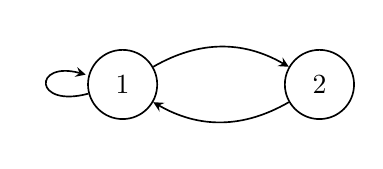
\begin{tikzpicture}[->, >=stealth, auto, semithick, node distance=2.5cm, scale=0.8]
    \node[state] (1) {$1$};
    \node[state] (2) [right of=1] {$2$};
    \path (1) edge[loop left] node{} (1)
          (1) edge[bend left] node{} (2)
          (2) edge[bend left] node{} (1);
\end{tikzpicture}
\end{center}
\end{column}
\begin{column}{0.5\textwidth}
\begin{center}
\textbf{Periodisch} ($d=2$):\\[0.3cm]
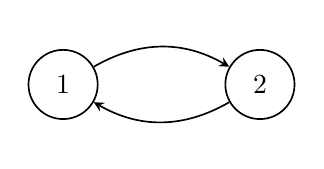
\begin{tikzpicture}[->, >=stealth, auto, semithick, node distance=2.5cm, scale=0.8]
    \node[state] (1) {$1$};
    \node[state] (2) [right of=1] {$2$};
    \path (1) edge[bend left] node{} (2)
          (2) edge[bend left] node{} (1);
\end{tikzpicture}
\end{center}
\end{column}
\end{columns}
\vspace{0.3cm}
\textbf{Hinweis:} Eine Selbstschleife ($p_{ii} > 0$) garantiert stets $d(i)=1$.
 \end{frame}


%% =============================================
%% BEISPIEL PERIODISCH
%% =============================================

\begin{frame}
    \frametitle{Markov-Ketten}
\framesubtitle{Beispiel: Periodische Kette}
    \begin{block}{Beispiel mit 2 Zuständen}
\[
P = \begin{pmatrix} 0 & 1 \\ 1 & 0 \end{pmatrix}
\]
\end{block}
Die Kette springt \emph{immer} zwischen den Zuständen hin und her:
\[
1 \to 2 \to 1 \to 2 \to \ldots
\]
\pause
\begin{itemize}
\item Rückkehr zu Zustand 1 nur nach $2, 4, 6, \ldots$ Schritten.
\item $d(1) = \gcd\{2, 4, 6, \ldots\} = 2$. \quad $\Rightarrow$ Periodisch!
\item Die invariante Verteilung ist $\pi = (1/2, 1/2)$, aber $P^n$ konvergiert \textbf{nicht}!
\end{itemize}
 \end{frame}


%% =============================================
%% LEAN: PERIODISCHES BEISPIEL
%% =============================================

\begin{frame}[fragile]
    \frametitle{Markov-Ketten}
\framesubtitle{Lean -- Periodisches Beispiel}
    \begin{block}{Periodische Kette in Lean}
\begin{verbatim}
def periodicP : S 2 -> S 2 -> Real
  | <0, _>, <0, _> => 0  | <0, _>, <1, _> => 1
  | <1, _>, <0, _> => 1  | <1, _>, <1, _> => 0

def periodicPi : S 2 -> Real
  | <0, _> => 1/2
  | <1, _> => 1/2

lemma periodicPi_isInvariant :
    IsInvariant periodicP periodicPi := by
  intro j
  fin_cases j <;>
    simp [periodicP, periodicPi,
          Fin.sum_univ_two] <;> ring
\end{verbatim}
\end{block}
$\pi = (1/2, 1/2)$ ist invariant, aber $P^n$ oszilliert!
 \end{frame}


%% =============================================
%% HAUPTSATZ: EXISTENZ UND EINDEUTIGKEIT
%% =============================================

\begin{frame}
    \frametitle{Markov-Ketten}
\framesubtitle{Hauptsatz über invariante Verteilungen}
    \begin{block}{Satz (Existenz und Eindeutigkeit)}
Sei $(X_n)$ eine \textbf{irreduzible} Markov-Kette mit endlichem Zustandsraum $S$. Dann gilt:
\begin{enumerate}
\item Es existiert \textbf{genau eine} invariante Verteilung $\pi$.
\item $\pi_i > 0$ für alle $i \in S$.
\item Ist die Kette zusätzlich \textbf{aperiodisch}, so gilt für jede Anfangsverteilung $\mu_0$:
\[
\lim_{n \to \infty} \mu_0 P^n = \pi
\]
d.h. die Verteilung konvergiert gegen $\pi$, unabhängig vom Startzustand.
\end{enumerate}
\end{block}
 \end{frame}


%% =============================================
%% LEAN: HAUPTSATZ STATEMENT
%% =============================================

\begin{frame}[fragile]
    \frametitle{Markov-Ketten}
\framesubtitle{Lean -- Hauptsatz (Statement)}
    \begin{block}{Formales Statement in Lean}
\begin{verbatim}
theorem stationary_unique
    (P : S N -> S N -> Real)
    (hP : IsTransitionMatrix P)
    (hirr : IsIrreducible P)
    (pi1 pi2 : S N -> Real)
    (hpi1_dist : IsDistribution pi1)
    (hpi2_dist : IsDistribution pi2)
    (hpi1_inv : IsInvariant P pi1)
    (hpi2_inv : IsInvariant P pi2) :
    pi1 = pi2
\end{verbatim}
\end{block}
\pause
\begin{block}{Beweis-Strategie}
Definiere $f = \pi_1 - \pi_2$. Dann ist $f$ harmonisch ($Pf = f$) und $\sum f_i = 0$. Das Maximumsprinzip + Irreduzibilität erzwingt $f = 0$.
\end{block}
 \end{frame}


%% =============================================
%% BEWEIS TEIL 1: EXISTENZ
%% =============================================

\begin{frame}
    \frametitle{Markov-Ketten}
\framesubtitle{Beweis -- Teil 1: Existenz}
    \begin{block}{Existenz einer invarianten Verteilung}
Betrachte die Cesàro-Mittel der Übergangsmatrizen:
\[
\overline{P}_n := \frac{1}{n} \sum_{k=0}^{n-1} P^k
\]
\end{block}
\pause
\begin{itemize}
\item Da $S$ endlich ist, liegt jede Zeile von $\overline{P}_n$ in einem kompakten Raum (Simplex der Wahrscheinlichkeitsvektoren).
\pause
\item Nach dem Satz von Bolzano-Weierstraß existiert eine konvergente Teilfolge $\overline{P}_{n_k} \to Q$.
\pause
\item Jede Zeile $q_i$ von $Q$ ist ein Wahrscheinlichkeitsvektor mit $q_i \cdot P = q_i$:
\[
\overline{P}_n \cdot P = \frac{1}{n} \sum_{k=0}^{n-1} P^{k+1} = \overline{P}_n + \frac{1}{n}(P^n - I) \to Q
\]
Also $Q \cdot P = Q$, d.h. jede Zeile von $Q$ ist invariant.
\end{itemize}
 \end{frame}


%% =============================================
%% BEWEIS TEIL 2: POSITIVITÄT
%% =============================================

\begin{frame}
    \frametitle{Markov-Ketten}
\framesubtitle{Beweis -- Teil 2: $\pi_i > 0$ für alle $i$}
    \begin{block}{Alle Einträge von $\pi$ sind positiv}
Sei $\pi$ eine invariante Verteilung und $i \in S$ beliebig.
\end{block}
\pause
\begin{itemize}
\item Da die Kette irreduzibel ist, gibt es für jedes $j$ mit $\pi_j > 0$ ein $m \geq 1$ mit $p_{ji}^{(m)} > 0$.
\pause
\item Aus $\pi = \pi P^m$ folgt:
\[
\pi_i = \sum_{k \in S} \pi_k \cdot p_{ki}^{(m)} \geq \pi_j \cdot p_{ji}^{(m)} > 0
\]
\pause
\item Da mindestens ein $\pi_j > 0$ existieren muss ($\pi$ ist Wahrscheinlichkeitsvektor), folgt $\pi_i > 0$ für alle $i$.
\end{itemize}
 \end{frame}


%% =============================================
%% LEAN: POSITIVITÄT
%% =============================================

\begin{frame}[fragile]
    \frametitle{Markov-Ketten}
\framesubtitle{Lean -- Positivität}
    \begin{block}{Schlüssel-Lemma: $\pi = \pi P^n$}
\begin{verbatim}
lemma invariant_of_pow (P : S N -> S N -> Real)
    (pi : S N -> Real) (hInv : IsInvariant P pi) :
    forall n, forall j, (Sum i, pi i * matPow P n i j) = pi j
\end{verbatim}
\end{block}
\pause
\begin{block}{Positivität}
\begin{verbatim}
theorem stationary_pos (P : S N -> S N -> Real)
    (hP : IsTransitionMatrix P)
    (hirr : IsIrreducible P) (pi : S N -> Real)
    (hpi_dist : IsDistribution pi)
    (hpi_inv : IsInvariant P pi) :
    forall i, 0 < pi i
\end{verbatim}
Beweis: $\exists\, j$ mit $\pi_j > 0$.  Irreduzibilität liefert $n$ mit $P^n_{ji} > 0$. \\
Dann $\pi_i = \sum_k \pi_k P^n_{ki} \geq \pi_j P^n_{ji} > 0$.
\end{block}
 \end{frame}


%% =============================================
%% BEWEIS TEIL 3: EINDEUTIGKEIT
%% =============================================

\begin{frame}
    \frametitle{Markov-Ketten}
\framesubtitle{Beweis -- Teil 3: Eindeutigkeit}
    \begin{block}{Die invariante Verteilung ist eindeutig}
Angenommen, $\pi$ und $\tilde{\pi}$ sind zwei invariante Verteilungen.
\end{block}
\pause
Definiere $f := \pi - \tilde{\pi}$. Dann gilt:
\begin{itemize}
\item $f \cdot P = f$ \quad (Differenz zweier Fixpunkte ist Fixpunkt)
\item $\sum_i f_i = 1 - 1 = 0$
\end{itemize}
\pause
Sei $i^* = \arg\max_i f_i$. Aus $f = fP$ folgt:
\[
f_{i^*} = \sum_j p_{i^* j} f_j \leq f_{i^*} \cdot \underbrace{\sum_j p_{i^* j}}_{= 1} = f_{i^*}
\]
Gleichheit gilt nur, wenn $f_j = f_{i^*}$ für alle $j$ mit $p_{i^* j} > 0$.
 \end{frame}


\begin{frame}
    \frametitle{Markov-Ketten}
\framesubtitle{Beweis -- Teil 3: Eindeutigkeit (Fortsetzung)}
    \begin{block}{Schluss per Irreduzibilität}
Wir haben gezeigt: $f_j = f_{i^*}$ für alle $j$ mit $p_{i^*j} > 0$.
\end{block}
\pause
\begin{itemize}
\item Wiederhole das Argument: Wenn $f_j = f_{i^*}$ und $p_{jk} > 0$, dann auch $f_k = f_{i^*}$.
\pause
\item Da die Kette \textbf{irreduzibel} ist, kann man von $i^*$ jeden Zustand $k \in S$ in endlich vielen Schritten erreichen.
\pause
\item Also: $f_k = f_{i^*}$ für \textbf{alle} $k \in S$.
\pause
\item Da $\sum_k f_k = 0$ und alle $f_k$ gleich sind: $|S| \cdot f_{i^*} = 0$, also $f_{i^*} = 0$.
\pause
\item Damit $f = 0$, d.h. $\pi = \tilde{\pi}$. \hfill $\square$
\end{itemize}
 \end{frame}


%% =============================================
%% LEAN: EINDEUTIGKEIT
%% =============================================

\begin{frame}[fragile]
    \frametitle{Markov-Ketten}
\framesubtitle{Lean -- Maximumsprinzip \& Eindeutigkeit}
    \begin{block}{Harmonische Funktionen}
\begin{verbatim}
def IsHarmonic (P : S N -> S N -> Real) (f : S N -> Real) :=
  forall x, stepOp P f x = f x

theorem harmonic_const_of_irreducible
    (P : S N -> S N -> Real) (hP : IsTransitionMatrix P)
    (hirr : IsIrreducible P)
    (f : S N -> Real) (hf : IsHarmonic P f) :
    forall i j, f i = f j
\end{verbatim}
\end{block}
\pause
\begin{block}{Beweisstruktur}
$f$ harmonisch $\Rightarrow$ $f(i^*) = \sum_j P_{i^* j} f(j)$, wobei $f(i^*) = \max f$.\\
Da $f(i^*) \geq f(j)$ und Konvexkombination: $f(j) = f(i^*)$ für $P_{i^*j}>0$.\\
Irreduzibilität propagiert dies auf alle $j \in S$.
\end{block}
 \end{frame}


%% =============================================
%% BEWEIS TEIL 4: KONVERGENZ
%% =============================================

\begin{frame}
    \frametitle{Markov-Ketten}
\framesubtitle{Beweis -- Teil 4: Konvergenz (Skizze)}
    \begin{block}{Bei Aperiodizität: $P^n \to \Pi$ (alle Zeilen = $\pi$)}
\end{block}
\pause
\begin{itemize}
\item Definiere den \textbf{Variationsabstand}: $\|u - v\|_{TV} = \frac{1}{2}\sum_i |u_i - v_i|$.
\pause
\item Für jede Zeile $e_i P^n$ (Verteilung nach $n$ Schritten, Start in $i$):
\[
\|e_i P^n - \pi\|_{TV} = \|e_i P^{n} - \pi P^n\|_{TV} \leq \|e_i - \pi\|_{TV} \cdot \rho^n
\]
wobei $\rho < 1$ (Kontraktionseigenschaft bei Irreduzibilität + Aperiodizität).
\pause
\item Da $\rho^n \to 0$: Konvergenz gegen $\pi$ für jede Anfangsverteilung. \hfill $\square$
\end{itemize}
 \end{frame}


%% =============================================
%% KONVERGENZ BEISPIEL
%% =============================================

\begin{frame}
    \frametitle{Markov-Ketten}
\framesubtitle{Konvergenz -- Beispiel}
    \begin{block}{Wetter-Beispiel: Potenzen von $P$}
\[
P = \begin{pmatrix} 0.8 & 0.2 \\ 0.4 & 0.6 \end{pmatrix}, \quad
P^5 \approx \begin{pmatrix} 0.672 & 0.328 \\ 0.656 & 0.344 \end{pmatrix}, \quad
P^{20} \approx \begin{pmatrix} 0.667 & 0.333 \\ 0.667 & 0.333 \end{pmatrix}
\]
\end{block}
\pause
\begin{itemize}
\item Die Zeilen von $P^n$ konvergieren beide gegen $\pi = (2/3, 1/3)$.
\item Egal ob Start in Sonne oder Regen -- langfristig gleiche Verteilung!
\end{itemize}
\pause
\begin{block}{Numerische Verifikation}
$\pi P = (2/3, 1/3) \begin{pmatrix} 0.8 & 0.2 \\ 0.4 & 0.6 \end{pmatrix} = (2/3 \cdot 0.8 + 1/3 \cdot 0.4, \; 2/3 \cdot 0.2 + 1/3 \cdot 0.6) = (2/3, 1/3) \;\checkmark$
\end{block}
 \end{frame}


%% =============================================
%% BEISPIEL 3 ZUSTÄNDE: INVARIANTE VERTEILUNG
%% =============================================

\begin{frame}
    \frametitle{Markov-Ketten}
\framesubtitle{Beispiel: Invariante Verteilung (3 Zustände)}
    \begin{block}{Stimmungs-Modell}
\[
P = \begin{pmatrix} 0.5 & 0.4 & 0.1 \\ 0.3 & 0.4 & 0.3 \\ 0.2 & 0.3 & 0.5 \end{pmatrix}
\]
Gesucht: $\pi = (\pi_G, \pi_N, \pi_S)$ mit $\pi P = \pi$, $\pi_G + \pi_N + \pi_S = 1$.
\end{block}
\pause
Gleichungssystem:
\begin{align*}
0.5\pi_G + 0.3\pi_N + 0.2\pi_S &= \pi_G \\
0.4\pi_G + 0.4\pi_N + 0.3\pi_S &= \pi_N \\
\pi_G + \pi_N + \pi_S &= 1
\end{align*}
\pause
Lösung: $\pi = \left(\frac{1}{3}, \frac{11}{30}, \frac{3}{10}\right) \approx (0.333, \; 0.367, \; 0.300)$
 \end{frame}


%% =============================================
%% DETAILED BALANCE (REVERSIBILITÄT)
%% =============================================

\begin{frame}
    \frametitle{Markov-Ketten}
\framesubtitle{Detailed Balance -- Reversibilität}
    \begin{block}{Definition (Detailed Balance)}
Eine Verteilung $\pi$ erfüllt die \textbf{Detailed-Balance-Bedingung} bzgl. $P$, falls:
\[
\pi_i \cdot p_{ij} = \pi_j \cdot p_{ji} \quad \text{für alle } i, j \in S
\]
\end{block}
\pause
\begin{block}{Satz}
Erfüllt $\pi$ die Detailed-Balance-Bedingung, so ist $\pi$ invariant.
\end{block}
\pause
\begin{block}{Beweis}
\[
(\pi P)_j = \sum_i \pi_i p_{ij} = \sum_i \pi_j p_{ji} = \pi_j \underbrace{\sum_i p_{ji}}_{=1} = \pi_j \quad \checkmark
\]
\end{block}
\textbf{Interpretation:} Im Gleichgewicht ist der ``Fluss'' von $i$ nach $j$ gleich dem Fluss von $j$ nach $i$.
 \end{frame}


%% =============================================
%% LEAN: DETAILED BALANCE
%% =============================================

\begin{frame}[fragile]
    \frametitle{Markov-Ketten}
\framesubtitle{Lean -- Detailed Balance}
    \begin{block}{Definition und Satz in Lean}
\begin{verbatim}
def DetailedBalance (P : S N -> S N -> Real)
    (pi : S N -> Real) : Prop :=
  forall i j, pi i * P i j = pi j * P j i

theorem detailedBalance_implies_invariant
    (hP : IsTransitionMatrix P)
    (hdb : DetailedBalance P pi) :
    IsInvariant P pi := by
  intro j
  calc Sum i, pi i * P i j
      = Sum i, pi j * P j i := by
        congr 1; ext i; exact hdb i j
    _ = pi j * Sum i, P j i := by
        rw [Finset.mul_sum]
    _ = pi j := by rw [hP.2 j, mul_one]
\end{verbatim}
\end{block}
Dieser Beweis ist in Lean \textbf{vollständig} -- kein \texttt{sorry}!
 \end{frame}


%% =============================================
%% DETAILED BALANCE BEISPIEL
%% =============================================

\begin{frame}
    \frametitle{Markov-Ketten}
\framesubtitle{Detailed Balance -- Beispiel}
    \begin{block}{Wetter-Beispiel: Prüfe Detailed Balance}
$\pi = (2/3, 1/3)$, \quad $P = \begin{pmatrix} 0.8 & 0.2 \\ 0.4 & 0.6\end{pmatrix}$
\end{block}
\pause
Prüfe $\pi_S \cdot p_{SR} = \pi_R \cdot p_{RS}$:
\[
\frac{2}{3} \cdot 0.2 = \frac{2}{15} \qquad \text{und} \qquad \frac{1}{3} \cdot 0.4 = \frac{2}{15} \quad \checkmark
\]
\pause
$\Rightarrow$ Das Wetter-Modell ist \textbf{reversibel}.

\vspace{0.3cm}
\textbf{Nicht jede Kette ist reversibel!} Beispiel: Kreislauf $1 \to 2 \to 3 \to 1$ mit
\[
P = \begin{pmatrix} 0 & 1 & 0 \\ 0 & 0 & 1 \\ 1 & 0 & 0 \end{pmatrix}
\]
hat $\pi = (1/3, 1/3, 1/3)$, aber $\pi_1 p_{12} = 1/3 \neq 0 = \pi_2 p_{21}$.
 \end{frame}


%% =============================================
%% ZUSAMMENFASSUNG
%% =============================================

\begin{frame}
    \frametitle{Markov-Ketten}
\framesubtitle{Zusammenfassung}
    \begin{block}{Zentrale Begriffe}
\begin{itemize}
\item \textbf{Markov-Kette:} Zukunft hängt nur von Gegenwart ab.
\item \textbf{Stochastische Matrix:} Zeilensummen $= 1$, Einträge $\geq 0$.
\item \textbf{Invariante Verteilung:} $\pi P = \pi$ (Gleichgewicht).
\item \textbf{Irreduzibel:} Jeder Zustand von jedem erreichbar.
\item \textbf{Aperiodisch:} Keine periodischen Zyklen.
\end{itemize}
\end{block}
\pause
\begin{block}{Hauptsatz}
\textbf{Irreduzibel + endlich} $\Rightarrow$ es existiert genau eine invariante Verteilung $\pi > 0$.\\
\textbf{+ Aperiodisch} $\Rightarrow$ Konvergenz: $P^n \to$ Matrix mit Zeilen $\pi$.\\[0.2cm]
Alle Definitionen und Beweise sind in Lean 4 / Mathlib formalisierbar!\\
Siehe: \texttt{code/LeanMath/stochastic/markov\_invariant.lean}
\end{block}
 \end{frame}


\end{document}
